\documentclass{article}

\usepackage{arxiv}

\usepackage[utf8]{inputenc} % allow utf-8 input
\usepackage[T1]{fontenc}    % use 8-bit T1 fonts
\usepackage{lmodern}        % https://github.com/rstudio/rticles/issues/343
\usepackage{hyperref}       % hyperlinks
\usepackage{url}            % simple URL typesetting
\usepackage{booktabs}       % professional-quality tables
\usepackage{amsfonts}       % blackboard math symbols
\usepackage{nicefrac}       % compact symbols for 1/2, etc.
\usepackage{microtype}      % microtypography
\usepackage{graphicx}

\title{Responsible Repositories}

\author{
    Nathanael Sheehan
   \\
    College of Engineering, Mathematics and Physical Sciences \\
    Exeter University \\
  University of Exeter, St Germans Road, EX4 7HD Exeter, UK \\
  \texttt{\href{mailto:ns651@exeter.ac.uk}{\nolinkurl{ns651@exeter.ac.uk}}} \\
   \And
    Sabina Leonelli
   \\
    EGENIS, Centre For The Study Of Life Sciences \\
    Exeter University \\
  University of Exeter, St Germans Road, EX4 7HD Exeter, UK \\
  \texttt{\href{mailto:s.leonelli@exeter.ac.uk}{\nolinkurl{s.leonelli@exeter.ac.uk}}} \\
  }


% tightlist command for lists without linebreak
\providecommand{\tightlist}{%
  \setlength{\itemsep}{0pt}\setlength{\parskip}{0pt}}



\begin{document}
\maketitle


\begin{abstract}
In this paper I aruge on the importance of TRUST
\end{abstract}

\keywords{
    SARS-CoV2
   \and
    Open Science
   \and
    Data Governance
  }

\hypertarget{introduction}{%
\section{Introduction}\label{introduction}}

The effectiveness of disseminating results promptly, sometimes even
before having them formally published -- thereby speeding up research -
has been extolled by scientific and popular media alike, most evidently
in relationto the prompt dissemination of genetic sequencing data from
various strains of the SARSCOV-2 virus (an exemplary instance of `Open
Data') and the decision by publishing companies to temporarily release
all coronavirus-related papers without charges (`Open Access'). As the
United Nations joins the choir of OS supporters with its 2021
recommendation to implement OS worldwide, the OS movement looks
well-positioned to determine the future of post-pandemic research and
related policies. This shift in research practice - in conjunction with
decreasing costs in data storage - has led to the latest research
findings, treatments and protocols on Covid-19 and related topics
becoming freely avalalible on the internet.

Belief in misinformation about COVID-19 poses a potential risk to public
health; therefore, scientists play a key role as disseminators of
factual and reliable information (Roozenbeek et al., 2020) In an Open
Science context, the TRUST (Transparency, Responsibility, User Focus,
Sustainability, and Technology ) principles highlight a set of
guidelines to demonstrate the trustworthiness of a digital repository to
many of the stakeholders involved, including researchers, community
users, funders, developers and service providers. ``Trustworthiness is
demonstrated through evidence, which depends on transparency, and thus
repositories must provide transparent, honest, and verifiable evidence
of their practice. In this way, stakeholders can be confident that
repositories ensure data integrity, authenticity, accuracy, reliability,
and accessibility over extended time frames. Trustworthiness is not a
one-off achievement; it cannot be taken for granted without regular
audit and certification'' (Lin et al 2020)

\hypertarget{method}{%
\section{Method}\label{method}}

propose metric for evaluating ``R,'' as done with FAIR principles

\hypertarget{discussion}{%
\section{Discussion}\label{discussion}}

\begin{enumerate}
\def\labelenumi{(\arabic{enumi})}
\setcounter{enumi}{2}
\item
  suggest that this metric is insufficient or anyhow ambiguous, because
  it takes no account of an additional and central factor in assessing
  responsibility: i.e.~underpinning interpretation of what counts as
  responsible openness
\item
  suggest that this should be added as a crucial additional factor for
  R, BUT also that this cannot be easily transformed into a binary
  metric (1-0) -- we are looking at qualitative differences
\item
  discuss how this works out in case og GISAID vs COVID-19 portal: here
  we have a clash of ideologies and experiences of what constitutes
  ``good'' openness
\end{enumerate}

\hypertarget{conclusion}{%
\section{Conclusion}\label{conclusion}}

\begin{enumerate}
\def\labelenumi{(\arabic{enumi})}
\setcounter{enumi}{5}
\tightlist
\item
  conclusion: there is much that CAN be done to metricise and evaluate
  TRUST principles as a key complement to FAIR, however even such
  evaluation needs to highlight the unavoidable
  qualitative/interpretative differences in the implementation of
  openness
\end{enumerate}

Repository

R1.1 Complete Metadata

R1.2 Techincal Documentation

R1.3 Quality Control

R1.4 Authenticity Protection

R2.1 Reliable Data Services

R3.1 Manage IP of Data Producers

R3.2 Security of System \& Content

Score

{GISAID }

{0.5}

{0.5}

{1}

{1}

{1.0}

{1}

{0.5}

{5.5}

{Covid-19 Data Platform}

{0.5}

{0.5}

{1}

{0}

{0.5}

{0}

{0.5}

{3.0}

Albiet, TRUST is not a new concept and a number of trustworthiness
certification mechanisms already exist; The Open Archival Information
System (OAIS) provides a recommendation model to provide long-term
preservation and access to digital information{[}REF{]}. The FAIR
principles emphasize a best practice of machine and human re-usability
with data objects.

\hypertarget{methods}{%
\section{Methods}\label{methods}}

\begin{figure}
\centering
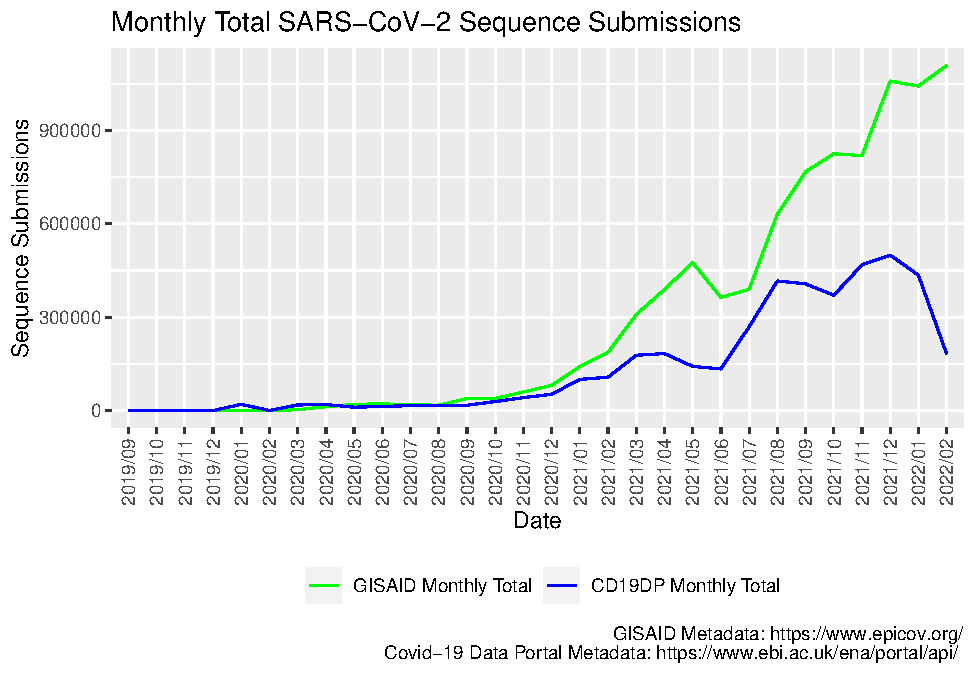
\includegraphics{Report_files/figure-latex/fig2-1.pdf}
\caption{Monthly totals of global SARS-CoV-2 cases sequenced and shared
on the GISAID and Covid-19 Data Platform database until Febuary 22 2022}
\end{figure}

\bibliographystyle{unsrt}
\bibliography{references.bib}


\end{document}
